\documentclass[a4paper, openany]{memoir}

\usepackage[utf8]{inputenc}
\usepackage[T1]{fontenc} 
\usepackage[english]{babel}

\usepackage{fancyhdr}
\usepackage{float}

\usepackage{amsmath}
\usepackage{amsthm}
\usepackage{amssymb}
\usepackage{enumitem}
\usepackage{multicol}
\usepackage[bookmarksopen=true,bookmarksopenlevel=2]{hyperref}
\usepackage{tikz}
\usepackage{indentfirst}

\usepackage{listings}
\usepackage{xcolor}

\pagestyle{fancy}
\fancyhf{}
\fancyhead[LE]{\leftmark}
\fancyhead[RO]{\rightmark}
\fancyhead[RE, LO]{WAD}
\fancyfoot[LE, RO]{\thepage}
\fancyfoot[RE, LO]{Pete Gautam}

\definecolor{ocre}{RGB}{52,177,201}
\definecolor{ultramarine}{RGB}{0,45,97}
\definecolor{mybluei}{RGB}{0,0,255}
\definecolor{myblueii}{RGB}{100,0,100}
\definecolor{myblueiii}{RGB}{50,234,253}

\definecolor{codegreen}{rgb}{0,0.6,0}
\definecolor{codegray}{rgb}{0.5,0.5,0.5}
\definecolor{codepurple}{rgb}{0.58,0,0.82}
\definecolor{backcolour}{rgb}{0.95,0.95,0.92}

\lstdefinestyle{mystyle}{
    backgroundcolor=\color{backcolour},   
    commentstyle=\color{codegreen},
    keywordstyle=\color{blue},
    numberstyle=\tiny\color{codegray},
    stringstyle=\color{codepurple},
    basicstyle=\ttfamily\footnotesize,
    breakatwhitespace=false,         
    breaklines=true,                 
    captionpos=b,                    
    keepspaces=true,                 
    numbers=left,                    
    numbersep=5pt,                  
    showspaces=false,                
    showstringspaces=false,
    showtabs=false,                  
    tabsize=2
}
\lstset{style=mystyle}


\lstdefinelanguage{XML}{
    sensitive=false, 
    keywords={
        xml, breakfast_menu, food, name, price, calories,
        DOCTYPE, ELEMENT, note, to, from, heading, body,
        xs, complexType, sequence, type,
        employees, employee, firstName, lastName,
    },  
    ndkeywords={},  
    morecomment=[s]{<!--}{-->},
    stringstyle=\color{purple}\ttfamily,
    morestring=[b]',
    morestring=[b]"
}

\lstdefinelanguage{JavaScript}{
  keywords={typeof, new, true, false, catch, function, return, null, try, catch, finally, switch, var, if, in, while, do, else, case, break, document, class, this, export, boolean, throw, implements, import},
  keywordstyle=\color{blue}\bfseries,
  ndkeywords={},
  ndkeywordstyle=\color{darkgray}\bfseries,
  identifierstyle=\color{black},
  sensitive=false,
  comment=[l]{//},
  morecomment=[s]{/*}{*/},
  commentstyle=\color{purple}\ttfamily,
  stringstyle=\color{red}\ttfamily,
  morestring=[b]',
  morestring=[b]"
}

\renewcommand{\headrulewidth}{1.5pt}

\chapterstyle{thatcher}

\begin{document}
    \chapter{Web Development}

    \section{Introduction to Web App Development}
    There are many web applications, e.g. Instagram, Twitter, Wikipedia, Skype, Amazon, etc. Formally, a web application is a distributed information management (DIM) system. It enables the management, sharing, finding, modification and presentation of information. That is, we can think of a web application in terms of the information it has- it is sharing the information, allowing people to search and edit it, and showing it in an appropriate manner. The web application does so over a network, in a distributed fashion. It typically has many users, often separated geographically.

    Ideally, DIMs enable users to access timely, relevant and useful information in a seamless manner. The users should not be able to view the complexity behind the app.

    There are two types of architecture in web development: system and information architecture. System architecture builds the infrastructure of the DIM syst-em- all the bits of technology and how they interact with each other. Information architecture is concerned with structuring and categorising information- it involves creating an environment for clients and users to interact with the system.

    The system architecture is system-focused. The design elements for system architecture include: specification and requirements; high-level system architecture; entity-relationship diagrams; and sequence diagrams. On the other hand, information architecture is user-focused. The design elements for information architecture include: user personas; user needs matrix; site and URL design; wireframes and walkthroughs.

    \subsection{System Components}
    At high level, the system architecture we have is:
    \begin{center}
        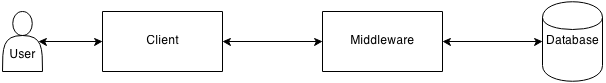
\includegraphics[scale=0.8]{src/L1I1.png}
    \end{center}
    In the diagram, the user is someone who is accessing a web application. The client is the device with which we access the application. The middleware links the client to the databases. In this course, we use the middleware Django. Typically, the middleware isn't running in the user's device. The web browser is running on their phone, but the middleware is not. The database is where the hosted data lives. This could be on a different server. The arrows represent that there is a two-way communication between the two entities.

    The user could be a human or a machine. They initiate contact and interact with the client. They range in skills and abilities. They have a number of requirements that need to be satisfied. 

    The client is a program sitting on a client device (e.g. a web browser). It sends request messages, e.g. to load the page or to post an image. It accepts response messages, e.g. the content of the web page that the browser will render to the user. It acts on the message- it can either communicate this message to the user (e.g. an alert message), or it affects the environment in some way (e.g. increase temperature).

    The request message is sent from the client to server. This could be to ask for some information, or to send some information to be stored. This information could either come from user input, or from some device (e.g. a sensor).

    The response message is sent from the server to a client. It can return the requested information or create some change within the environment.

    The request message protocol is typically an HTTP request. It can be embedded in any data to be sent, e.g. XML or JSON. The response message protocol is an HTTP response. It returns content that is often in XML or JSON.

    The middleware/application server is the central component. It can accept request messages from clients. It can return response messages. It coordinates the application components. The backend/database is typically on a separate node. It stores the data for the application. It provides the data when needed. It needs to be scalable and reliable. It could be a database, an index or a flat file.

    \subsection{Web Development Complexity}
    There are many languages involved in web development. These include markup languages (e.g. HTML and XML), programming languages (e.g. Java-Script) and database query languages (e.g. SQL). With Django, we do not need to use SQL heavily- it uses an ORM, and Django abstracts SQL. This means that we can interact with SQL directly through Python.

    There are also shifting standards in web development. The DOM, XML and JSON have standards associated with them, but these standards evolve over time. We need to keep up with these changes.

    The browsers themselves evolve over time. The browser wars encourage them to come up with new, unique features. We also need to keep up with these. While we can make use of these features in some browsers, we still need to make our web app compatible with all the browsers. This is another challenge.

    Moreover, HTTP is a stateless protocol. It doesn't keep track of variables or values in the memory. Each request between the client and the server is executed independently with no association with the previous behaviour. So, if we wanted the site to save password/remember some user preferences, then there is nothing inherent in HTTP that allows us to do so. Nonetheless, most applications require the persistence of state.

    However, there are signs of hope. Web development has become a serious business. Despite all the challenges, there are many incentives to persevere. In line with this, the methods of development are maturing. We are increasingly adopting the good practices of `classical' software engineering for native app development. These rely on application-programmer interfaces (APIs), libraries, frameworks, standards and tools.

    \subsection{Web Development Tools}
    The nature of web development is disjoint. The developer must become familiar with a set of distinct and (typically) non-integrated tools. Web development tool support is not yet as advanced as with `classic' software development. Most languages have several complex integrated complex development environments (IDEs) to choose from. These include IDLE, Eclipse, PyCharm, etc.

    An important tool is the text editor or IDE. The choice of the text editor and our expertise in its usage can seriously affect our productivity. It has syntax awareness, auto-completeness, snippets, scripts and macros, along with integration with other development tools. Some IDEs have plugins for scripting languages, e.g. Eclipse has a PHP plug-in.

    Interpreted languages lack the compilation stage where errors and warnings can be raised. Frustratingly, scripts will just run until they reach an error and fail over. If we ware lucky, we might get an error message. But, it won't make sense most of the time. There are however a wide range of tools that will perform static analysis of scripts to spot errors, e.g. PyLint/JSLint, PHP\_CodeSniffer, chrome's developer tools, firebug for firefox, etc.

    There are also W3C (World Wide Web Consortium) standards. Each aspect of the software is specified by a W3C activity run by a working group which produces the following reports:
    \begin{itemize}
        \item working draft- no consensus yet;
        \item candidate recommendation- published in order to gather implementation experience and feedback;
        \item proposed recommendation- sent for final approval by advisory committee;
        \item w3C recommendation- approved by the W3C.
    \end{itemize}
    This also means that everything is constantly evolving.

    \subsection{Development Environment}
    \subsubsection{Command-line interfaces}
    Using command-line interfaces, we can control software or an operating system by issuing text-based commands. This is an alternative to Graphical User Interface (GUI). An operating system might have both, and we can use either one. It can be used to perform many common tasks, such as navigate around directory (folder) structure, create and edit files, run applications, and so on.

    In Anaconda Prompt, the following are few common commands:
    \begin{itemize}
        \item \texttt{dir}, which lists files in the current directory (\texttt{ls} on UNIX-based OS).
        \item \texttt{mkdir <name>}, which creates a new directory with the provided \texttt{name}.
        \item \texttt{cd <name>}, which changes directory and navigates to the provided destination \texttt{name}.
        \item \texttt{cd ..}, which moves `up' one level to the current directory's parent.
    \end{itemize}
    We will also have a look at some django, anaconda and git-specific commands later.

    It is a good software practice to:
    \begin{itemize}
        \item use a version control system, e.g. git;
        \item use a package manager, e.g. pip;
        \item use a virtual environment, e.g. Anaconda;
        \item use an IDE, e.g. PyCharm, IDLE, VS code.
    \end{itemize}

    \subsubsection{Version Control System- Github}
    There are many version control systems such as CVS, subversion, Mercurial, git, etc. It maintains a history of a software project. It is often remotely-stored. Multiple users can contribute to code. It is common practice in industry and open projects to use version control. It is essential for teams, but also useful for individual projects.

    There are many advantages to using version control. It gives access to older (working) versions of the code. We can keep track of different versions and releases. It greatly simplifies concurrent work. We can compare and understand changes made by others. It enables changes to be easily merged. It safeguards the code against some disaster, especially if the repository is in the cloud. It enables exploratory work, i.e. branching.

    We now focus on git. It is one of the newer version control systems which has some benefits over the older ones. It has efficient and flexible controls. There is an `extra step' of a local repository. This allows for easier branching and encourages more commits.

    The following diagram explains how git data transport works.
    \begin{center}
        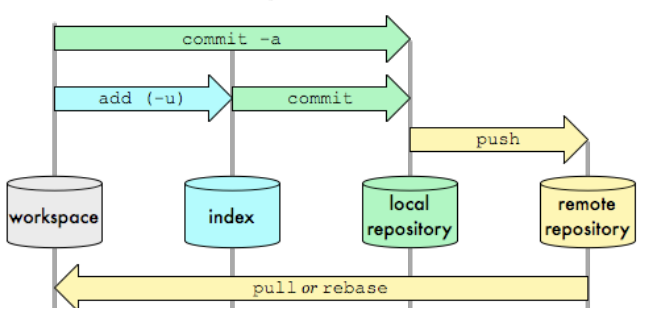
\includegraphics[scale=0.6]{src/L2I1.png}
    \end{center}
    First, we note that there are 4 areas- the workspace, index, local repository and remote repository. It is only the remote repository that isn't present locally; everything else lies on the computer. 

    The workspace is composed of the local files (i.e. the folder). We want to take snapshots of the workspace and send them to the repository. 

    The snapshots are then stored in a local repository. This is an extra stage that other version control systems don't have. This means that we do not need to connect to the internet to use the command; it encourages more commits. Also, it means that the commit doesn't affect other people's work.

    The index is an extra stage that many version controls don't have. This is where we state what we want to commit (whenever that happens). It gives us extra control on what we want to commit. Most of the times, we want to commit everything. However, this command gives us more flexibility in the committing process.

    The command \texttt{git clone} creates a local copy of a project from a remote link. Any subsequent update can be done by the \texttt{git pull} command.

    The command \texttt{git add} adds the new files updated in the workspace to the index. These are the files that will get committed when the time comes. The command \texttt{git add *} adds all the files in the workspace.

    The command \texttt{git status} shows us the files that are at index and the changes made to the workspace.

    After adding the files to the index, we run the command \texttt{git commit} to add all these files to our local repository. The command \texttt{git commit -a} runs both \texttt{git add -u} and \texttt{git commit}, however this does not add the new files committed.

    Finally, the command \texttt{git push} sends all the content from our local repository to the remote repository. The code is now available in github.

    If we were starting from scratch and wanted to create a git repository, we can either clone a repo that already exists on a remote host, or start using git with an existing project in our computer. To clone a repo, we use the command \texttt{git clone <url>}, where the \texttt{url} is the github url of the code. 
    To create a repo from our own code, we can type in the following commands:
    \begin{itemize}
        \item \texttt{git init} to initialise git; 
        \item \texttt{git add *} to add all the files to the index;
        \item \texttt{git commit -m "first commit"} to commit from the index to the local repo;
        \item \texttt{git remote add origin <url>} to connect this project with the github project at the provided \texttt{url}; 
        \item and then \texttt{git push -u origin master} to finally push to the remote \newline repository.
    \end{itemize}

    \subsubsection{Package Manger- Pip}
    Package managers are software tools that automate the process of installing, upgrading and configuring software libraries. It turns the packages installed and their dependencies. If the pre-requisite packages are not installed, it will install them too. 

    They help overcome the nightmare of managing libraries, setting up software and replicating an environment. The list of packages is defined. It is easy to install the same set of libraries and versions multiple times. It is stored in the package manager and exportable.

    Pip is a popular package manager for Python. Pip is used to install and manage packages from PyPi (python package index). Using pip reduces development set up hassles. We don't need to mess around with path issues. We don't need to worry about what version of the library is used as this is specified in the file. It is easy to export and share the `requirements', i.e. the set of libraries used. It is easy to install the same set of libraries on another machine. It works in conjunction with virtual environments.

    To install a package using pip, we use the command \texttt{pip install}. We can specify which version of the package we want, e.g. \texttt{pip install django==2.2.17}. The command \texttt{pip list} shows all the installed packages. Moreover, the command \texttt{pip freeze > requirements.txt} creates the file `requirements.txt' wi-th the list of packages within the workspace. The command \texttt{pip freeze} also shows all the installed packages.

    \subsubsection{Virtual Environment- Anaconda}
    A virtual environment instance is a local environment that is configured to provide access to libraries, settings, hardware. They keep the dependencies required by different projects in separate places. They don't interfere with each other or the system. Virtual environment software refers to an application that implements, manages and controls multiple virtual environment instances.

    Anaconda is a tool to keep the dependencies required by different projects in separate places. It isolates the different environments and lets us switch between them easily. It has the following advantages:
    \begin{itemize}
        \item We can separate package installations. We can use different package sets for each project.
        \item We can separate python versions. We can use different python versions for each project.
        \item Virtual environments can be created/switched between easily using the Anaconda command prompt.
    \end{itemize}

    The command \texttt{conda create -n <ENVNAME> python=3.8.5} creates an environment called \texttt{ENVNAME}. We do not need to specify the version of Python; if left blank, it would default to the version in the system.

    The command \texttt{conda activate <ENVNAME>} enters the \texttt{ENVNAME} environment.

    The command \texttt{conda deactivate} leaves the environment. Note that this has no parameters since we can only be in one environment at any time.

    The command \texttt{conda env list} lists all the environments present.

    The command \texttt{conda env remove -n <ENVNAME>} deletes the provided environment \texttt{ENVNAME}.
    \newpage

    \section{Introduction to HTML}
    Hyper-text markup language (HTML) is the language used by web browsers to interpret what gets displayed when we view a web page. A mark-up language is a set of tags that describe the content within the document. Hyperlinks are connections between the documents. HTML documents (i.e. web pages) contain HTML mark-up tags and plain text.

    The following is a basic HTML example:
\begin{lstlisting}[language=html]
<html>
<head>
    <title>Title</title>
</head>
<body>
    <h1>WAD2</h1><br>
    <p>Hello World</p>
</body>
</html>
\end{lstlisting}
    The page is made up of many tags. These are keywords (the names of the tag) surrounded by angle brackets \texttt{<>}. For example, line 1 features an \texttt{html} tag. Normally, we have opening and closing tags, e.g. the \texttt{html} tag in line 1 is an opening tag, while the \texttt{html} tag in line 9 is its closing tag.

    There is also plain text between tags, For example, line 7 has the plain text \texttt{Hello World}. This is the content displayed in the browser.

    HTML has nested tags. For example, the \texttt{head} tag in line 2 is nested within the \texttt{html} tag in line 1. Moreover, the \texttt{title} tag in line 3 is nested within the \texttt{head} tag in line 2. An HTML file starts with the \texttt{html} tag.

    Also, the \texttt{html} tag only has two children- the \texttt{head} and the \texttt{body} tag, and these are presented in this order. The \texttt{head} tag contains information about the document, e.g. the title and meta tags. These are the content not displayed within the web page. The \texttt{body} tag contains the html that is displayed within the web page.

    An element is the content from an opening tag to the corresponding closing tag, including the tags themselves. For example, line 6 features the element \texttt{<h1>WAD2</h1>}. Moreover, the \texttt{body} itself is an element, containing lines 5-8. The plain text between the opening and the closing tags is called the element content. So, the content in line 6 is \texttt{WAD2}.

    There are also some tags which have no content. They also have no tag, e.g. the \texttt{br} tag in line 6. This command forces a line break in the document.

    We have the tag \texttt{h1} (header 1) in line 6. It should only be used once and defines the most important heading. Search engines use the tag \texttt{h1} to determine the content of the web page. There are 6 header tags: \texttt{h1}, \texttt{h2}, up to \texttt{h6}. The tag \texttt{h1} renders the most important header.

    We have the tag \texttt{p} (paragraph) in line 7. Browser add space before and after each \texttt{<p>} element. The browser ignores the formatting provided in the HTML- the whitespace is collapsed.

    We can create hyperlinks with \texttt{a} (anchor) tags. For example,
\begin{lstlisting}[language=html]
Go to <a href="https://google.co.uk">Google</a>
\end{lstlisting}
    The \texttt{href} within the \texttt{a} tag is called an attribute. In this case, the value of the attribute is the link \texttt{https://google.co.uk}.

    We can create an unordered list of items, which is rendered with bullet points. We make use of the tags \texttt{ul} and \texttt{li}, as shown below:
\begin{lstlisting}[language=html]
<ul>
    <li>List item one</li>
    <li>List item two</li>
</ul>
\end{lstlisting}

    A \texttt{div} tag allows us to create sections to divide the page in different ways when coupled with CSS.

    A \texttt{span} tag is used to group inline-elements in a document, again when coupled with CSS. For example,
\begin{lstlisting}[language=html]
<p>I have<span style="color:blue">blue</span>eyes.</p>
\end{lstlisting}
    The text would render as: `I have {\color{blue}blue} eyes.`. If we used a \texttt{div} tag instead, then the text would be rendered in 3 lines since the tag triggers a line break.
    \newpage

    \section{Overview of Django}
    We consider the high-level system architecture diagram again to consider how to start creating a web application.
    \begin{center}
        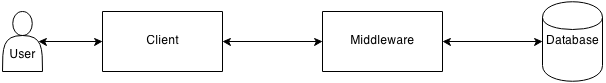
\includegraphics[scale=0.8]{src/L1I1.png}
    \end{center}
    First, we need to work out what we are going to build. Then, we need to decide what technologies will be used in each box. For the middleware, we will be fixing Django as the Web Application Framework (WAF) for building the application server.

    Django is a high-level Python web framework that encourages rapid development and clean, pragmatic design. It primarily focuses on dynamic and databa-se-driven websites, content based websites. Many large sites have used Django before, e.g. Instagram, Spotify, WaPo, Dropbox, etc.

    Django lets us divide a site or code module into logical components. It is underpinned by the MVC/MTV design pattern. It provides flexibility and makes it easier to use. It provides automatically generated web administration. This makes it easier to manage the database. It also provides many pre-packaged APIs for common tasks.

    Django also provides a template system to define the HTML templates. They avoid code duplications and subscribe to the DRY (don't repeat yourself) principle. It gives us extra control to define what the URL will be for a given view. The URL requested by browser is not directly accessing the html file. It makes use of a loose coupling principle. It also allows us to separate logic from presentation- this is called the separation of concerns.

    The following are the design philosophies in Django:
    \begin{itemize}
        \item Use loose coupling- the various layers of the framework don't need to `kn-ow' about each other in detail (unless absolutely necessary);
        \item Don't repeat yourself (DRY)- every piece of knowledge must have a single, unambiguous, authoritative representation within a system;
        \item Write less Code;
        \item Develop fast;
        \item Explicit is better than implicit- this is a core Python principle;
        \item Aim for consistency.
    \end{itemize}
    Django has many modules to acheive many tasks such as administration interface (create, read, update and delete- CRUD), authentication systems, form and session handling, syndication frameworks (RSS and Atom feeds), Caching, internationalisation and localisation, etc.

    \subsection{Model View Controller}
    Model View Controller (MVC) is a software-architectural design pattern. It divides the software into three interconnected parts and achieves a separation of concerns. The models describe the internal data representation. The view determine what the user sees. The controller binds it all together, handles logic and interactions. This is not a firm definition; individual `MVC' designs vary significantly.

    In Django, the model describes the database entities and relationships. They are specified as Python classes. The views are specified using web templating. The controller is handled by the Django framework and the URL parser. The URL parser maps the urls to the views. These definitions are not concrete. 

    Django has objects called `views' that query and process data, and might be considered part of the controller role in MVC. Some people include templates in describing the structure of Django, so MVCT (model, view, controller, template) or MTV (model, template, view).

    The (simplified) internal flow of Django is:
    \begin{center}
        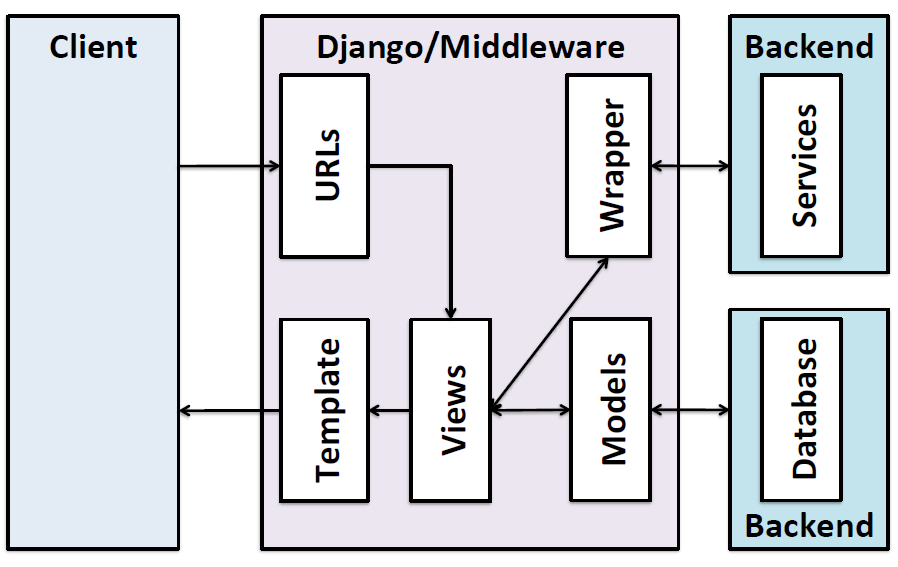
\includegraphics[scale=0.6]{src/L3I1.PNG}
    \end{center}
    The data models (in \texttt{models.py}) specify the entities and relationships in the database. These provide an Object-Relational Mapping (ORM) to the actual database tables. The framework constructs the database given the models. In Django, the database is SQL.

    The views (in \texttt{views.py}) are responsible for handling and processing the specific request. It collates the data from databases and external services. We then select the template for the response to be generated.

    We control flow through \texttt{urls.py}. To specify what view function should handle a particular URL (or part thereof), URL patterns are used to find matches with the URL, and to route this request to the appropriate view. The use of pattern matching means that different instantiations can be handled by a common pattern.

    The templates specify the response format (html, xml, etc.) is decoupled from the data to be presented.

\end{document}